\documentclass[a4paper,11pt]{article}
\usepackage{graphicx}
\graphicspath{ {../graphs/} }

\begin{document}
\title{Lab1 Report}
\author{Kailean O'Keefe}
\date{\today}
\maketitle

\section*{Introduction}
This assignment was all about simulating the flow of traffic on a simple network. It shows in depth how packets are transferred over a connection, and discusses various scenarios where information can be held up, as well as why information is held up while being transferred. 

\section*{Two Nodes}
a) These were the network files that I used in this simulation:
\begin{verbatim}
--------------------
FAST-LONG

n1 n2
n2 n1

n1 n2 1Mbps 1000ms
n2 n1 1Mbps 1000ms
--------------------
SLOW-SHORT

n1 n2
n2 n1

n1 n2 100bps 10ms
n2 n1 100bps 10ms
--------------------
FAST-SHORT

n1 n2
n2 n1

n1 n2 1Mbps 10ms
n2 n1 1Mbps 10ms
\end{verbatim}
b) Here is the output of the full simulation:
\begin{verbatim}
********Scenario 1********
(1, 0, 1, 1.008, 1)
********Scenario 2********
(1, 0, 1, 80.01, 1)
********Scenario 3********
(1, 0, 1, 0.018000000000000002, 1)
(2, 0, 2, 0.026000000000000002, 2)
(3, 0, 3, 0.034, 3)
(4, 2000.0, 4, 2000.018, 4)
\end{verbatim}
c) Finally, here are the calculations to show that the above results are accurate:\\
Scenario 1: $d_t = L/R+d_p$ $((1000*8)/1000000) + 1$ = 1.08\\
Scenario 2: $d_t = L/R+d_p$ $((1000*8)/100) + .01$ = 80.01\\
Scenario 3: $d_t = L/R+d_p$ $((1000*8)/1000000) + .01$ = .018\\

\section*{Three Nodes}
a) These were the network files that I used in this simulation:
\begin{verbatim}
--------------------
FAST-FAST

n1 n2 
n2 n1 n3 
n3 n2

# link configuration
n1 n2 1Mbps 100ms
n2 n3 1Mbps 100ms

n2 n1 1Mbps 100ms
n3 n2 1Mbps 100ms
--------------------
FASTER-FASTER

n1 n2 
n2 n1 n3 
n3 n2

# link configuration
n1 n2 1Gbps 100ms
n2 n3 1Gbps 100ms

n2 n1 1Gbps 100ms
n3 n2 1Gbps 100ms
--------------------
FAST-SLOW

n1 n2 
n2 n1 n3 
n3 n2

# link configuration
n1 n2 1Mbps 100ms
n2 n3 256Kbps 100ms

n2 n1 1Mbps 100ms
n3 n2 256Kbps 100ms
\end{verbatim}
b) Here is the output of the last five lines of the simulation:
\begin{verbatim}
********Scenario 1********
(996, 107460.0, 996, 107460.21599999999, 996, 0.21599999998579733,
  996, 0.016, 996, 0.2, 996, 0.0, 996)
(997, 107568.0, 997, 107568.21599999999, 997, 0.21599999998579733, 997, 
  0.016, 997, 0.2, 997, 0.0, 997)
(998, 107676.0, 998, 107676.21599999999, 998, 0.21599999998579733, 998,
  0.016, 998, 0.2, 998, 0.0, 998)
(999, 107784.0, 999, 107784.21599999999, 999, 0.21599999998579733, 999,
  0.016, 999, 0.2, 999, 0.0, 999)
(1000, 107892.0, 1000, 107892.21599999999, 1000, 0.21599999998579733, 1000,
  0.016, 1000, 0.2, 1000, 0.0, 1000)
********Scenario 2********
(996, 107460.0, 996, 107460.20001599999, 996, 0.20001599998795427, 996,
  1.6e-05, 996, 0.2, 996, 0.0, 996)
(997, 107568.0, 997, 107568.20001599999, 997, 0.20001599998795427, 997,
  1.6e-05, 997, 0.2, 997, 0.0, 997)
(998, 107676.0, 998, 107676.20001599999, 998, 0.20001599998795427, 998,
  1.6e-05, 998, 0.2, 998, 0.0, 998)
(999, 107784.0, 999, 107784.20001599999, 999, 0.20001599998795427, 999,
  1.6e-05, 999, 0.2, 999, 0.0, 999)
(1000, 107892.0, 1000, 107892.20001599999, 1000, 0.20001599998795427, 1000,
  1.6e-05, 1000, 0.2, 1000, 0.0, 1000)
********Scenario 3********
(996, 107460.0, 996, 107460.23925, 996, 0.23924999999871943, 996,
  0.03925, 996, 0.2, 996, 0.0, 996)
(997, 107568.0, 997, 107568.23925, 997, 0.23924999999871943, 997,
  0.03925, 997, 0.2, 997, 0.0, 997)
(998, 107676.0, 998, 107676.23925, 998, 0.23924999999871943, 998,
  0.03925, 998, 0.2, 998, 0.0, 998)
(999, 107784.0, 999, 107784.23925, 999, 0.23924999999871943, 999,
  0.03925, 999, 0.2, 999, 0.0, 999)
(1000, 107892.0, 1000, 107892.23925, 1000, 0.23924999999871943, 1000,
  0.03925, 1000, 0.2, 1000, 0.0, 1000)
\end{verbatim}
c) Here are the equations that were used in obtaining that output:\\
Scenario 1: $d_t = L/R+d_p$ $((80000000)/2000000) + .1$ = 0.016\\
Scenario 2: $d_t = L/R+d_p$ $((80000000)/2000000000) + .1$ = 1.6e-05\\
Scenario 3: $d_t = L/R+d_p$ $((1000*8)/1000000) + ((80000000)/256000) + .1$ = 0.03925\\

\section*{Queuing Theory}
a) This was the network file that I used in this simulation:
\begin{verbatim}
--------------------
FAST-FAST

n1 n2 
n2 n1 n3 
n3 n2

# link configuration
n1 n2 1Mbps 100ms
n2 n3 1Mbps 100ms

n2 n1 1Mbps 100ms
n3 n2 1Mbps 100ms
\end{verbatim}
The data here shows that as the stream of packets coming into a node gets more sporadic -- or as $\lambda$ goes up, the queueing delay for each packet increases exponentially. This is shown by the graph below.\\
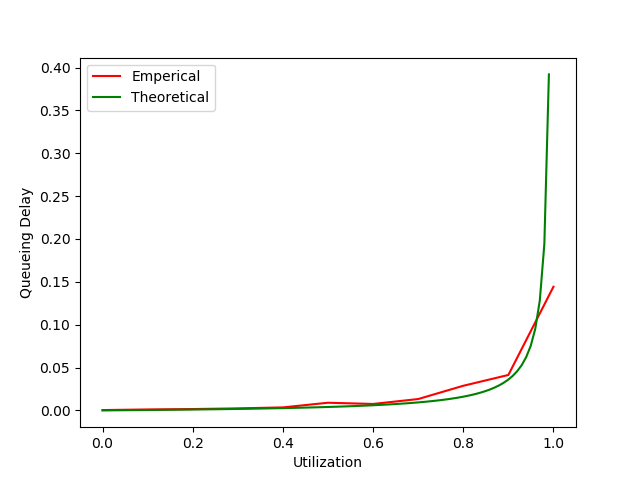
\includegraphics{graph}
As shown by the graph, the data generated by running the simulation very closely matches the predicted curve of the graph based off of the formula \[w = \frac{\rho}{(2\mu)(1-\rho)}\]  

\section*{Conclusion}
As shown above it is very important to be mindful of the various limitations that network transfers can have and to plan for them accordingly. If there are multiple hops in a network then it is important to make sure that the speeds between the various nodes are consistent, otherwise the connection can build up some very serious delays. It is also important to be mindful of the arrival rate of your packets. Even if your network is uniformly fast between its nodes, if packets are arriving sporadically the connection will take a significant hit in speed.

\end{document}
